% ------ headers globales -------------
\documentclass[11pt, a4paper, twoside]{article}
\usepackage{header}
\usepackage{config}
\usepackage{graphicx}
\usepackage{amsthm}
\usepackage[lined, boxed, commentsnumbered]{algorithm2e}
% -------------------------------------
\begin{document}

% -- Carátula --
%\clearpage{\pagestyle{empty}% **************************************************************************
%
%  Package 'caratula', version 0.3 (para componer caratulas de TPs del DC).
%
%  En caso de dudas, problemas o sugerencias sobre este package escribir a
%  Brian J. Cardiff (bcardif arroba gmail.com).
%  Nico Rosner (nrosner arroba dc.uba.ar).
%
% **************************************************************************

% ----- Informacion sobre el package para el sistema -----------------------

\NeedsTeXFormat{LaTeX2e}
\ProvidesPackage{caratula}[2005/08/09 v0.3 Para componer caratulas de TPs del DC]
\usepackage[pdftex]{graphicx}

% ----- Imprimir un mensajito al procesar un .tex que use este package -----

\typeout{Cargando package 'caratula' v0.3 (2005/08/09)}

% ----- Algunas variables --------------------------------------------------

\let\Materia\relax
\let\Submateria\relax
\let\Titulo\relax
\let\Subtitulo\relax
\let\Grupo\relax
\let\Fecha\relax
\let\Logoimagefile\relax
\let\Resumen\relax
\let\Tags\relax

% ----- Comandos para que el usuario defina las variables ------------------

\def\materia#1{\def\Materia{#1}}
\def\submateria#1{\def\Submateria{#1}}
\def\titulo#1{\def\Titulo{#1}}
\def\subtitulo#1{\def\Subtitulo{#1}}
\def\grupo#1{\def\Grupo{#1}}
\def\fecha#1{\def\Fecha{#1}}
\def\logoimagefile#1{\def\Logoimagefile{#1}}
\def\resumen#1{\def\Resumen{#1}}
\def\tags#1{\def\Tags{#1}}

% ----- Token list para los integrantes ------------------------------------

\newtoks\intlist\intlist={}

% ----- Comando para que el usuario agregue integrantes --------------------

\def\integrante#1#2#3{\intlist=\expandafter{\the\intlist
    \rule{0pt}{1.2em}#1&#2&\tt #3\\[0.2em]}}

% ----- Macro para generar la tabla de integrantes -------------------------

\def\tablaints{%
    \begin{tabular}[t]{| l @{\hspace{4ex}} c @{\hspace{4ex}} l|}
        \hline
        \multicolumn{1}{|c}{\rule{0pt}{1.2em} Integrante} & LU &  \multicolumn{1}{c|}{Correo electr\'onico} \\[0.2em]
        \hline \hline
        \the\intlist
        \hline
    \end{tabular}}

% ----- Codigo para manejo de errores --------------------------------------

\def\se{\let\ifsetuperror\iftrue}
\def\ifsetuperror{%
    \let\ifsetuperror\iffalse
    \ifx\Materia\relax\se\errhelp={Te olvidaste de proveer una \materia{}.}\fi
    \ifx\Titulo\relax\se\errhelp={Te olvidaste de proveer un \titulo{}.}\fi
    \edef\mlist{\the\intlist}\ifx\mlist\empty\se%
    \errhelp={Tenes que proveer al menos un \integrante{nombre}{lu}{email}.}\fi
    \expandafter\ifsetuperror}


% ----- \maketitletxt correspondiente a la versión v0.2 (texto) ---------

\def\maketitletxt{%
    \ifsetuperror\errmessage{Faltan datos de la caratula! Ingresar 'h' para mas informacion.}\fi
    \thispagestyle{empty}
    \begin{center}
    \vspace*{\stretch{2}}
    {\LARGE\textbf{\Materia}}\\[1em]
    \ifx\Submateria\relax\else{\Large \Submateria}\\[0.5em]\fi
    \par\vspace{\stretch{1}}
    {\large Departamento de Computaci\'on}\\[0.5em]
    {\large Facultad de Ciencias Exactas y Naturales}\\[0.5em]
    {\large Universidad de Buenos Aires}
    \par\vspace{\stretch{3}}
    {\Large \textbf{\Titulo}}\\[0.8em]
    {\Large \Subtitulo}
    \par\vspace{\stretch{3}}
    \ifx\Grupo\relax\else\textbf{\Grupo}\par\bigskip\fi
    \tablaints
    \end{center}
    \vspace*{\stretch{3}}
    \newpage}

% ----- \maketitle correspondiente a la versión v0.3 (gráfica) -------------

\def\maketitlegraf{%
    \ifsetuperror\errmessage{Faltan datos de la caratula! Ingresar 'h' para mas informacion.}\fi
%
    \thispagestyle{empty}

    \ifx\Logoimagefile\relax\else\includegraphics{\Logoimagefile}\fi \hfill \includegraphics{logo_dc.jpg}

    \vspace*{.07 \textheight}

    \noindent \textbf{\huge \Titulo}  \medskip \\
    \ifx\Subtitulo\relax\else\noindent\textbf{\large \Subtitulo} \\ \fi%
    \noindent \rule{\textwidth}{1 pt}

    {\noindent\large\Fecha \hspace*\fill \Materia} \\
    \ifx\Submateria\relax\else{\noindent \hspace*\fill \Submateria}\fi%

    \medskip%
    \begin{center}
        \ifx\Grupo\relax\else\textbf{\Grupo}\par\bigskip\fi
        \tablaints
    \end{center}%
    \bigskip
    %~ \ifx\Resumen\relax\else\textbf{\textsf{Resumen}} \\
    %~ \Resumen\bigskip\fi \\
    %~ \ifx\Tags\relax\else\textbf{\textsf{Palabras Clave}} \\
    %~ \Tags\par\bigskip\fi
    \vfill%
%
    \begin{minipage}[t]{\textwidth}
        \begin{minipage}[t]{.50 \textwidth}
            \includegraphics[width=0.9\textwidth]{logo_uba.jpg}
        \end{minipage}%%
        \begin{minipage}[b]{.55 \textwidth}
            \textbf{\textsf{Facultad de Ciencias Exactas y Naturales}} \\
            \textsf{Universidad de Buenos Aires} \\
            {\scriptsize %
            Ciudad Universitaria - (Pabell\'on I/Planta Baja) \\
                Intendente G\"uiraldes 2160 - C1428EGA \\
            Ciudad Aut\'onoma de Buenos Aires - Rep. Argentina \\
                Tel/Fax: (54 11) 4576-3359 \\
            http://www.fcen.uba.ar \\
            }
        \end{minipage}
    \end{minipage}%
%
    \newpage}

% ----- Reemplazamos el comando \maketitle de LaTeX con el nuestro ---------

\def\maketitle{\maketitlegraf}
\cleardoublepage}

%% =====================================================================

\clearpage
\section{Problema 3 - La comunidad del anillo}

\subsection{Descripción del problema a resolver}
La empresa \texttt{AlgoNET} nos contrató para que le brindemos una 
solución algorítmica a un problema de redes. Nuestro cliente quiere ofrecer
un sevicio particular sobre una red existente de computadoras. La red cuenta
con un conjunto de conexiones entre pares de computadoras, donde cada 
conexión tiene un costo asociado. El objetivo es elegir un subconjunto de 
conexiones y de equipos (que funcionarán como servidores) tales que:
\begin{enumerate}
  \item El conjunto de servidores deberá conformar un anillo
  \item Todo equipo debe quedar conectado al anillo de servidores vía un 
        enlace directo o pasando a través de otros equipos en el medio
  \item La suma total de los costos de todos los enlaces utilizados debe
        ser lomínimo posible
  \item El algoritmo debe tener una complejidad estrictamente mejor que $O(n^3)$
  \item El algoritmo debe detectar los casos en los que no haya solución
\end{enumerate}

El formato de entrada contiene una instancia del problema. La primera línea 
contiene un entero positivo $n$ que indica la cantidad de equipos de la red
(numerados de 1 a $n$), y un entero no negativo $m$ que corresponde a la 
cantidad de enlaces disponibles. A esta línea le siguen $m$ líneas, una para
cada enlace, con el formato \texttt{e1 e2 c} donde \texttt{e1} y \texttt{e2}
representan los equipos en lso extremos del enlace en cuestión (ambos enteros
entre 1 y $n$) y \texttt{c} es el costo por utilizar dicho enlace. En caso de
haber solución, la salida tiene el formato \texttt{C Ea Er} donde \texttt{C} es
el csoto de la solución dada y \texttt{Ea} y \texttt{Er} son los enlaces 
utilizados por el anillo y para el resto de la red, respectivamente. A esta línea
le siguen \texttt{Ea} líneas, una para cada enlace utilizado en el anillo y luego
\texttt{Er} líneas, una para cada enlace utilizado fuera del anillo, todas con el 
formato \texttt{e1 e2} donde \texttt{e1} y \texttt{e2} representan los extremos
del enlace en cuestión. Si hay más de una solución óptima, se puede devolver 
cualquier, y si no hay solución se debe devolver la palabra \texttt{no}. A 
continuación, mostramos un ejemplo de una posible instancia.

\begin{minipage}[t]{0.4\textwidth}
\begin{Verbatim}[frame=single,framesep=1cm,label= Ejemplo de entrada: instancia 1]
8 10
1 2 1
2 6 1
2 3 5
2 7 2
6 7 1
7 5 3
3 5 8
5 4 2
5 8 2
4 8 10
\end{Verbatim}
\end{minipage}
\hfill
\begin{minipage}[t]{0.4\textwidth}
\begin{Verbatim}[frame=single,framesep=1cm,label= Ejemplo de salida: instancia 1]
20 3 5
2 6
6 7
2 7
1 2
7 5
3 5
5 4
5 8
\end{Verbatim}
\end{minipage}

A continuación, presentamos una representación del problema, visto como 
un grafo: cada nodo es un equipo y cada arista es una conexión entre 
algún par de computadoras, y tiene un costo asociado a dicha conexión, 
seguido de tres posibles formas de elegir los subconjuntos de equipos y 
conexiones requeridos por el problema

\begin{figure}[H]
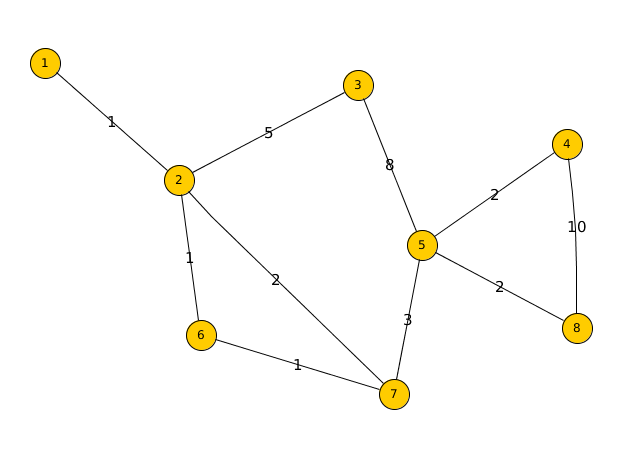
\includegraphics[scale=1]{imagenes/equipos2.png}
\caption{Red de equipos}
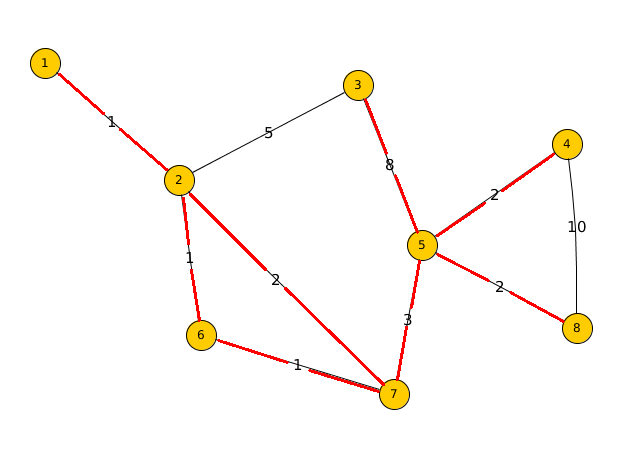
\includegraphics[scale=1]{imagenes/equipos3.png}
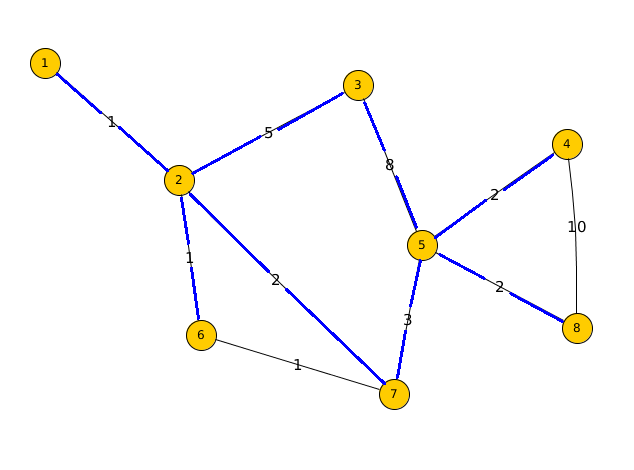
\includegraphics[scale=1]{imagenes/equipos4.png}
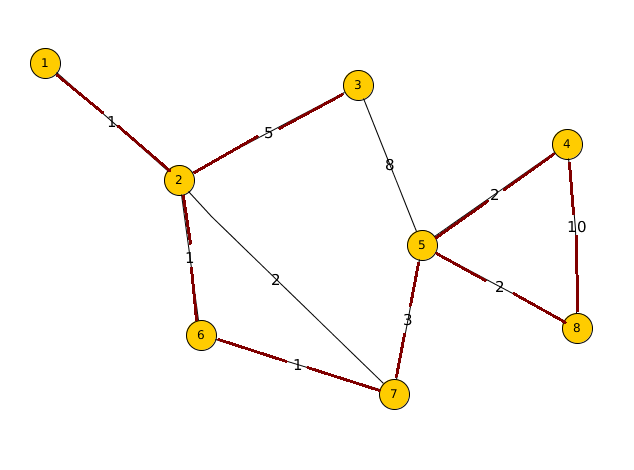
\includegraphics[scale=1]{imagenes/equipos5.png}
\caption{Soluciones de costo C = 20 (rojo), C = 24 (azul), C = 25 (marrón) respectivamente}
\end{figure}

Se puede observar que las tres soluciones presentadas en la figura 1.1.2 
son efectivamente soluciones porque todas presentan algún circuito de
servidores, y en todos los casos, todas las computadoras de la red están 
conectadas con los servidores con conexiones directas o a través de conexiones
con otros equipos. Sin embargo, no todas estas soluciones son óptimas: una 
tiene costo 20, otra 24 y otra 25. Es decir, que para este caso en particular,
nuestro algoritmo debería devolver como solución los servidores 2, 6, 7 y
los enlaces que están marcados en rojo en la figura 1.1.2.

\subsection{Ideas desarrolladas para la resolución}
A partir del ejemplo presentado en la sección anterior y de algunos otros,
observamos que en todos los casos, todos los enlaces que conformaban el 
árbol generador mínimo (AGM) del grafo generados por nuestra red de equipos
estaban incluidos en la solución óptima del problema. En nuestro ejemplo,
el AGM sería:

\begin{figure}[H]
\centering
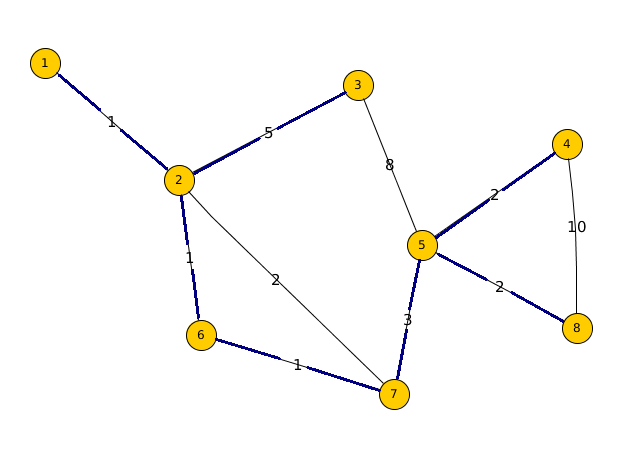
\includegraphics[scale=1]{imagenes/equipos6.png}
\caption{Árbol Generador Mínimo del grafo del ejemplo de la figura 1.1.1}
\end{figure} 

Entonces, pensamos que posiblemente esto siempre sucediera, al menos siempre
que existiera alguna solución. Así es que,
intentamos probar que tomando el AGM del grafo en cuestión y luego 
agregándole la arista de menor pero de las que no estuvieran incluidas
en el AGM, el grafo generado sería una solución (sería un grafo con algún 
ciclo y todos los nodos estarían conectados con algún nodo del conjunto de 
nodos que conformaban el ciclo en el grafo) y que sería óptima (la suma
total de los pesos de los enlaces sería lo mínimo posible). La demostración
está más adelante. \\
Entonces, a continuación describimos los pasos que nuestro algoritmo
efectuará para resolver el problema planteado:

\begin{enumerate}
  \item generar un grafo $G$ en donde cada nodo sea un equipo y cada arista un
        enlace entre un par de equipos, con un costo asociado igual al costo
        que hay que pagar por el ancho de banda empleado por dicha conexión
  \item chequear si el grafo $G$ es conexo. Si no lo es, entonces el problema
        no tendrá solución
  \item si el grafo $G$ es conexo, generar el árbol generador mínimo $T$ del grafo
        $G$
  \item buscar el menor de los enlaces que aparece en el grafo $G$ pero que no 
        aparece en el árbol generador mínimo $T$. Llamemos a ese eje $e$.
  \item agregamos el eje $e$ al AGM $T$. Queda así formado el grafo $G' = T + e$,
        que es un grafo conexo y tiene un único ciclo. Además, cumple con todo lo
        que nos pide el enunciado del problema
  \item devolvemos la suma total de los costos de todas las conexiones que son
        utilizadas por nuestro grafo $G'$ y, por otro lado, devolvemos los enlaces
        que conforman nuestro anillo de servidores y el resto de los enlaces 
        de nuestra solución
        
\end{enumerate}

\newpage
\subsection{Demostración de Correctitud}
Para demostrar la correctitud de nuestro algoritmo, tenemos que demostrar que los
pasos descriptos en la sección anterior para la resolución del problema 
efectivamente nos conducen a la generación de una solución correcta. Entonces,
repasando las ideas ya expuestas, lo que planteamos es que se puede llegar a una
solución óptima a partir de generar el AGM $T$ de nuestro grafo $G$ y luego generar
el grafo $G' = T + \{e\}$, donde $e$ es el eje de menor costo que esta en $G$ y
no en $T$. Pero lo que nos pide el enunciado es que generemos, a partir del grafo $G$,
otro grafo $G''$ tal que $G''$ sea conexo, contenga un único ciclo y que la suma
total de los costos de sus ejes sea lo mínima posible. Entonces, demostrando la 
siguiente proposición, estaríamos demostrando nuestro método empleado para la resolución
es efectivamente correcto:

\newtheorem{prop}{Proposición}
\begin{prop}
Dado un grafo G conexo, con T un AGM de G y S el conjunto de todos los árboles
generadores de G y $e$ el mínimo eje perteneciente a $G \backslash T$ vale que: 
$costo(T+e) = \min\limits_{\substack{f \in G \backslash T \\ T' \in S}} costo(T'+f)$
\end{prop}
\begin{proof}[Demostración de la Proposición 1] 
Primero, vamos a demostrar dos lemas: 
\begin{enumerate}
  \item si $S_{opt}$ es una solución óptima al problema (es algún subgrafo conexo  de G
		con algún ciclo), entonces $S_{opt}$ contiene a algún AGM de G.
		
		\begin{proof}[Demo de 1]
		Supongamos que $S_{opt}$ \textbf{no contiene} un AGM de G. Entonces, queremos ver que
		$S_{opt}$ no puede ser solución óptima para nuestro problema (hay alguna solución mejor).
		Claramente, si $S_{opt}$ contuviera algún AGM de G, entonces dicho árbol generador
		podría construirse tomando algún eje $e$ del ciclo que se forma en $S_{opt}$, y generando
		el grafo $G' = S_{opt} - \{e\}$. Pero, supongamos que al quitar cualquier eje $e$ del ciclo
		que se forma en $S_{opt}$, el árbol que queda no es un AGM. 
		\end{proof}
  
  \item dado un grafo G, si tomo algún AGM de G entonces la longitud de la mínima 
        arista de las que están en G $\backslash$ T es siempre la misma.
        
        \begin{proof}[Demo de 2]
		Supongamos que $T$ y $T'$ son dos AGM's distintos y que la arista de menor longitud 
		que queda en $G \backslash T$ es $e$ mientras que la de menor longitud que queda en
		$G \backslash T'$ es $f$ y además supongamos que peso($e$) $<$ peso ($f$). Entonces,
		como $T$ y $T'$ son árboles y están construidos sobre el mismo grafo $G$, sabemos que
		tienen la misma cantidad de aristas y $e \in T'$ pues de lo contrario $e$ sería el mínimo
		eje perteneciente a $G \backslash T'$ y no $f$.\\
		Ahora, supongamos que formamos el grafo 
		$H = T + \{e\}$. Se forma un ciclo: $e_{1}, e_{2} \dots e_{1}$, donde long($e$) $\geq$ 
		long($e_{i}$) (puesto que de lo contrario, podríamos obtener el árbol $T + \{e\} - \{e_{i}\}$, de 
		longitud menor que T) y además, \textbf{no todos} 
		los ejes $e_{i}$ están incluidos en $T'$, puesto que por hipótesis, $e \in T'$ y entonces
		$e$ formaría un ciclo en $T'$ con $e_{1} e_{2} \dots$, lo cual es absurdo porque $T'$ es un
		árbol y no puede tener ciclos.
		Luego, si $e_{k} \not\in T'$, como long($e_{k}$) $\leq$ long($e$) $<$ long($f$), $f$ no 
		era la arista más chica de $G \backslash T'$ (Absurdo). Entonces, concluimos que 
		peso($e$) $\geq$ peso($f$). Haciendo la misma demostración, pero con la hipótesis de que
		peso($f$) $<$ peso ($e$) obtendríamos exactamente la desigualdad opuesta. 
		Entonces, concluimos que peso($e$) $=$ peso ($f$) siempre, lo cual implica que 
		la longitud de la mínima arista de las que están en $G \backslash T$ tiene siempre de 
		la misma longitud, sin importar que AGM $T$ se elija.
		\end{proof}
\end{enumerate}
Entonces, si consideramos cualquier AGM $T$ de $G$, por lo demostrado en el punto 2, la
longitud de la mínima arista de las que quedan (llamémosla $e$) es siempre la misma.
Entonces, para cualquier AGM $T$ que elijamos, la longitud del grafo $ G'' = T + \{e\} $
también es siempre la misma, porque todos los AGM's de un grafo tienen que tener la misma
longitud. Entonces, sea $G_{opt}$ la solución óptima del problema para el grafo $G$. 
Por lo visto en el punto 1, $G_{opt}$ contiene un AGM de $G$. Supongamos que contiene 
al AGM $T$. Entonces, como además sabemos que $G_{opt}$ tiene un único ciclo, seguro que
$G_{opt} = T + \{e\}$ para algún eje $e$ que está en $G$ pero no en $T$. Pero para que 
$G_{opt}$ sea de longitud mínima, la longitud de $e$ debe ser menor o igual que la 
longitud de $f$ para cualquier eje $f \in G \backslash T$. Entonces, 
$G_{opt} = T + \{e\}$ donde $T$ es algún AGM de $G$ y $e$ es un eje perteneciente a
$G \backslash T$ y de longitud mínima en ese conjunto, y además la longitud de
$G_{opt} = T + \{e\}$ es siempre la misma, independientemente del AGM $T$ que hayamos
elegido. Esto es lo que queríamos demostrar.
\end{proof}

\newpage
\subsection{Justificación de cota de complejidad}

\begin{algorithm}[H]
\SetKwInOut{Input}{input}
\SetKwInOut{Output}{output}
  \Input{???}
  \Output{??}

\caption{Pseudocódigo para el algoritmo empleado en la resolución}
\end{algorithm}

\subsection{Testeos de complejidad}



%% =====================================================================

\end{document}
